%=========================================================================

%\documentclass[cover]{fitthesis}
\documentclass[a4paper,oneside,onecolumn,11pt]{report}

\usepackage[utf8]{inputenc}
\usepackage[english]{babel} 
\usepackage{url}
\usepackage[options, lined]{algorithm2e}
\usepackage{textcomp}
\usepackage{mathtools}
\usepackage{graphicx}
\usepackage{subfig}
\usepackage{amsmath}


\newcommand*{\titleAT}{\begingroup % Create the command for including the title page in the document
\newlength{\drop} % Command for generating a specific amount of whitespace
\drop=0.1\textheight % Define the command as 10% of the total text height

\rule{\textwidth}{1pt}\par % Thick horizontal line
\vspace{2pt}\vspace{-\baselineskip} % Whitespace between lines
\rule{\textwidth}{0.4pt}\par % Thin horizontal line

\vspace{\drop} % Whitespace between the top lines and title
\centering % Center all text
\textcolor{}{ % Red font color
{\Huge SYMBOLIC REGRESSION}\\[1.0\baselineskip] % Title line 1
{PROJECT FOR}\\[0.75\baselineskip] % Title line 2
{\Large ARTIFICIAL NEURAL NETWORKS}} % Title line 3

\vspace{0.25\drop} % Whitespace between the title and short horizontal line
\rule{0.3\textwidth}{0.4pt}\par % Short horizontal line under the title
\vspace{\drop} % Whitespace between the thin horizontal line and the author name

{\Large \textsc{Barbora Skrivankova}}\par % Author name

\vfill % Whitespace between the author name and publisher text
{\large \textcolor{}{\plogo}}\\[0.5\baselineskip] % Publisher logo
{\large \textsc{T.E.I. of Crete}}\par % Publisher

\vspace*{\drop} % Whitespace under the publisher text

\rule{\textwidth}{0.4pt}\par % Thin horizontal line
\vspace{2pt}\vspace{-\baselineskip} % Whitespace between lines
\rule{\textwidth}{1pt}\par % Thick horizontal line

\endgroup}


\begin{document}
\titleAT
\thispagestyle{empty}
\tableofcontents

\chapter{Introduction}
	This project was made as an year-end project for the theoretical part of the class Artificial
	Neural Networks on Department of Applied Informatics and Multimedia at Technical Eductional 
	Institute of Crete. The task was to find an application of neural networks on the internet, 
	and process it from a theoretical point of view. To introduce basic procedures which are
	done in order to get the result of neural network. \\

	The chosen application of neural networks is a diploma thesis from The Faculty of Applied Informatics
	on The University of Tomas Bata in Czech republic in Zlin. This thesis is dealing with analytical
	programming (special type of evolutionary algorithms) in order to make the optimalization of neural
	networks. It is comparing the algorithm SOMA (evolutionary type of algorithm) to the learning 
	process with backpropagation algorithm and nonlinear interlacing. I decided, that I will focus
	this project on the algorithm of backpropagation.\\

	Problem which is solved in this project is a symbolic regression, which is very popular in the world
	of artificial intelligence these days. As it is said on the website www.symbolicregression.com:
	"Symbolic regression is a function discovery approach for analysis and modeling of numeric multivariate 
	data sets for a purpose of getting insights about data-generating systems."\\

	There is a lot of researches focused on symbolic regression, one of them is taking place on my
	home university (Brno University of Technology), which is dealing with this problem by cartesian
	genetic programming, combined with coevolution. In the end of this project I am also comparing
	the results of neural networks to the results of cartesian genetic programming. After o comparsion
	of the performance on the basic symbolic regression problems, which were solved by neural networks
	in the mentioned thesis, I am trying to predict the success of neural networks on much more 
	difficult functions which I decided to use as testbenches in this theoretical project. \\

	I have chosen this topic mainly because of the topic my bachelor's thesis which is dealing with competitive
	coevolution in cartesian genetic programming applied to symbolic regression and its comparssion
	to coevolution of fitness predictors. Now, thanks to this project, I can also compare success of
	my algorithms t the success of neural networks in solving symbolic regression.
	

\chapter{Application description}
	The neural network which I am trying to describe in this project should be a neural
	network solving symbolic regression. Symbolic regression is a topic, which is now very
	popular in the field of artifical intelligence. We try to solve it not only with
	artifical neural networks, but also with genetic programming and genetic algorithms.\\

	In this chapter I am going to bring near the problematics of symbolic regression, approximate
	what do we expect from the general symbolic regression to do and how we will change it
	for the symbolic regression used in this project. Then, after the description of symbolic
	regression, I will introduce you the two functions which I chose for this project as a 
	test benchmarks. 

	\section{Symbolic regression}
	Symbolic regression is an approach to the function discovery. It is used for modeling
	and analyzing numerical data in order to get a purpose about data-generating systems. 
	As the name suggest, the method by which the insights are to be generated, is regression.\\

	The term symbolic regression is representing the process of interleaving some curve through
	the known data. This curve is usually expressed as a mathematical function. For a long time
	it used to be a qualification of humans only, but how time passes, it starts to be possible
	also with an artifical intelligence.\\

	Symbolic regression works as it is shown on the picture \ref{regrese}. As you can see on the left
	side, there is an input of symbolic regression, on the right side is the desired output.
	If we have a function, which takes one number (let's say $x$) as an input and gives us one 
	output (let's say $y$), we can logically organize this pairs into vectors $(x, y)$. If you
	have vectors in the shape of $(x, y)$, it is natural to draw it in a 2D plot like we can see 
	on the picture \ref{regrese}.\\

	\begin{figure}
		\centering
		\subfloat[][input of symbolic regression]{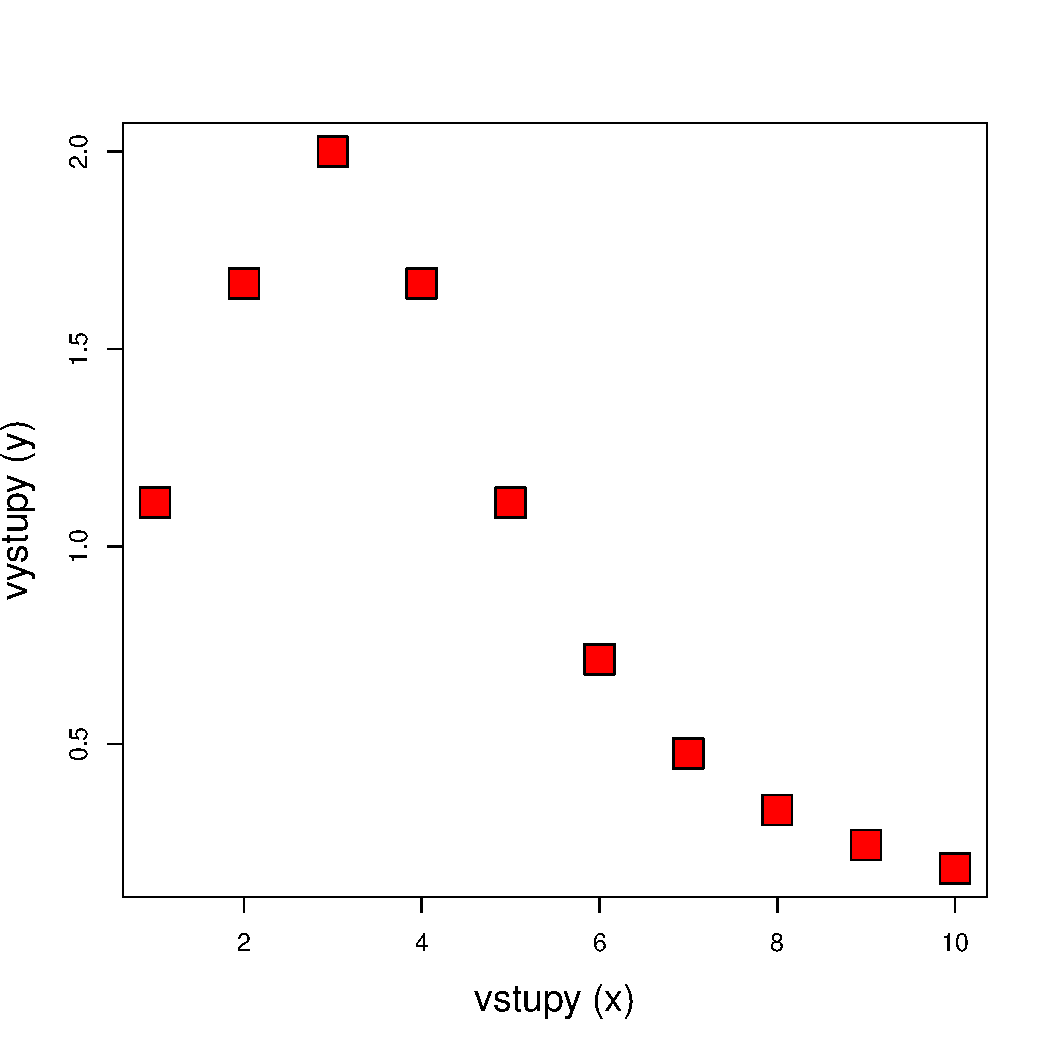
\includegraphics[width=60mm]{fig/points.pdf}}
		\subfloat[][output of symbolic regression]{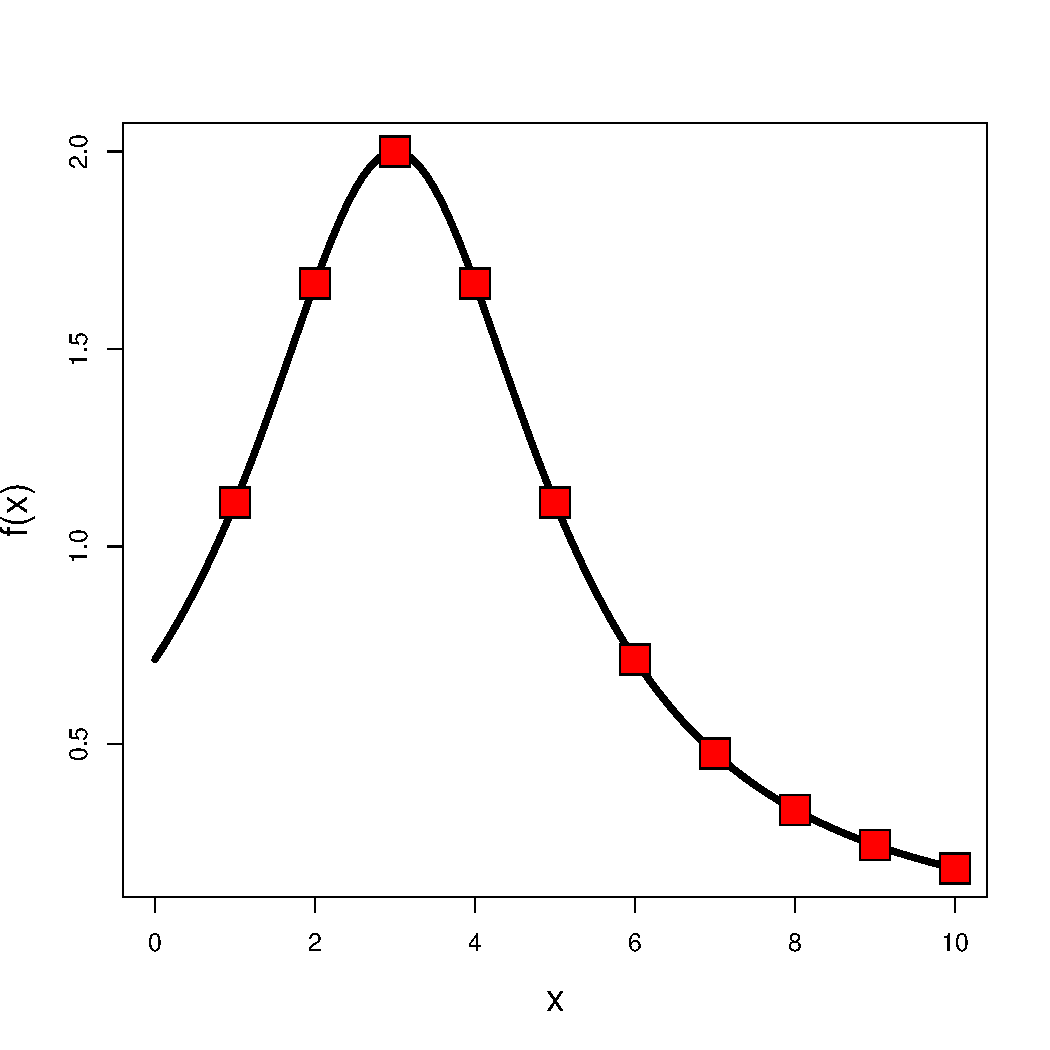
\includegraphics[width=60mm]{fig/regression.pdf}}
		\caption{Symbolic regression}
		\label{regrese}
	\end{figure}

	On the right side of the picture, we can see our desired output.
	We want the symbolic regression (or symbolic function identification) to find the some of the
	relations between the inputs and outputs. In more details, we need to identify which of the inputs
	is more important than other and how is it related to the changes in the output. In order 
	to predict, what would be the function value of some input which we didn't train the network on.
	In this example the value is always according to the function f as follows.

	\begin{equation}
		f(x) = \frac{10}{5 + (x - 3)^2}
	\end{equation}\\

	The goal of symbolic regression is in getting the relation between $x$ and $y$ onto whole 
	field of real numbers from our input, which are only vectors $(x_1, x_2, ...)$ identificating points in 
	the plane, space or multidimensional space, which the searched function goes through.\\

	As a demonstration of more difficult problem which can be solved by symbolic regression, I am adding another
	possible input displayed as a 3-dimensional plot (figure \ref{3d_input}. This plot is corresponding to the following function.

	\begin{equation}
		f(x_1, x_2) = \frac{(x_1 - 3)^4 + (x_2 - 3)^3 - (x_2 - 3)}{(x_2 - 2)^4 + 10}
	\end{equation}\\

	This function is also called rational polynomial function in 2 dimensions and is used in the community working
	on symbolic regression as a prove, that their algorithm can solve even the most challenging functions.

	\begin{figure}
		\centering
		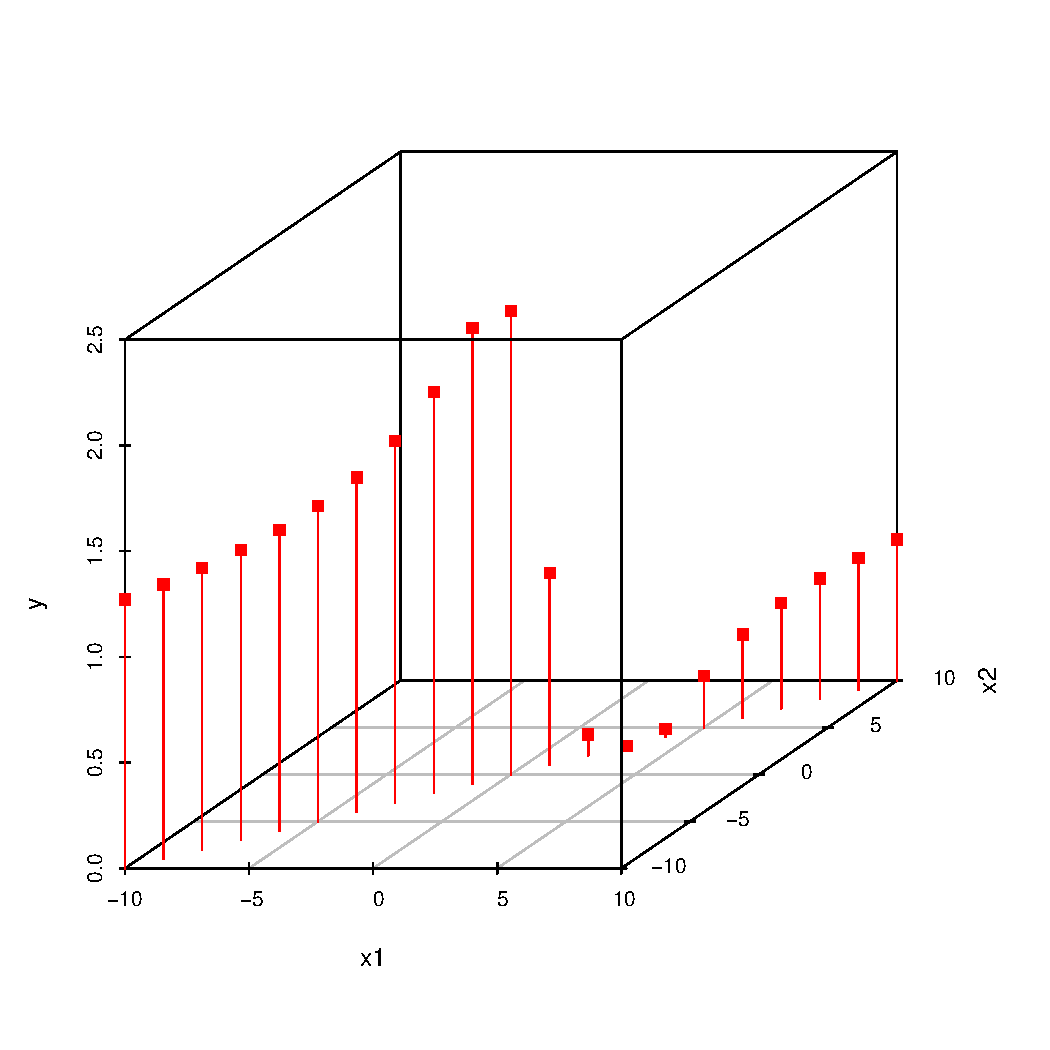
\includegraphics[width=90mm]{fig/3dfunc.pdf}
		\caption{Symbolic regression}
		\label{3d_input}
	\end{figure}

		\subsection{Our way of interpreting symbolic regression}
			For this project, we will want something little bit different from symbolic regression.
			Usualy we want it to tell us straightly the function in the shape of $y = f(x)$, 
			but here, in this project, we will not really want it to show us the function. We will want 
			the neural network to train to count all possible inputs of the function (in our case all
			the real numbers) and after, if we give it some input vector, which is not in the training
			patterns, we expect it to count the correct output. If we go deeper, we can imagine it
			as a formula inside the neural network, but we will not interpret it like this, we will 
			only wait for the outputs. 

	\section{Test benchmarks}
	\label{benchmarks}
		For symbolic regression we start from the basic tests with elementary functions (e.g.
		$y = x^2$) in the beginning to prove that the method is suitable to solve symbolic
		regression. As we already know, that symbolic regression is solvable with neural 
		networks (proven also in \cite{varacha2006}), we can continue in function discovery
		on more difficult functions. I decided to prepare two testing sets for two different
		functions to try the symbolic regression on them.\\

		I decided to use toy benchmarks from the website symbolicregression.com
		\footnote{http://symbolicregression.com/?q=node/5}, which is officialy the place
		where all the people from the community share their results, compare them to other
		results and check if their symbolic regression is properly working. The testbenches I 
		have concretely chosen from the symbolic regression website are testbench number 3: 
		Salustowitz function in 2 dimensions and testbench number 5: unwrapped ball function 
		in 2 dimensions.
		\subsection{Salustowitz function 3D}
			\begin{equation}
				f(x_1, x_2) = e^{-x_1} x_1^3 cos(x_1) sin(x_1) (cos(x_1) sin^2(x_1) - 1) (x_2 - 5)
			\end{equation}\\
			We can see the plot of the Salustowitz function on the figure \ref{salustowitz}, which is 
			plotted in the ranges as follow:
			\begin{equation}
				\begin{aligned}
				x_1 \in \langle 0, 10 \rangle\\
				x_2 \in \langle 0, 10 \rangle
				\end{aligned}
			\end{equation}

			\begin{figure}
				\centering
				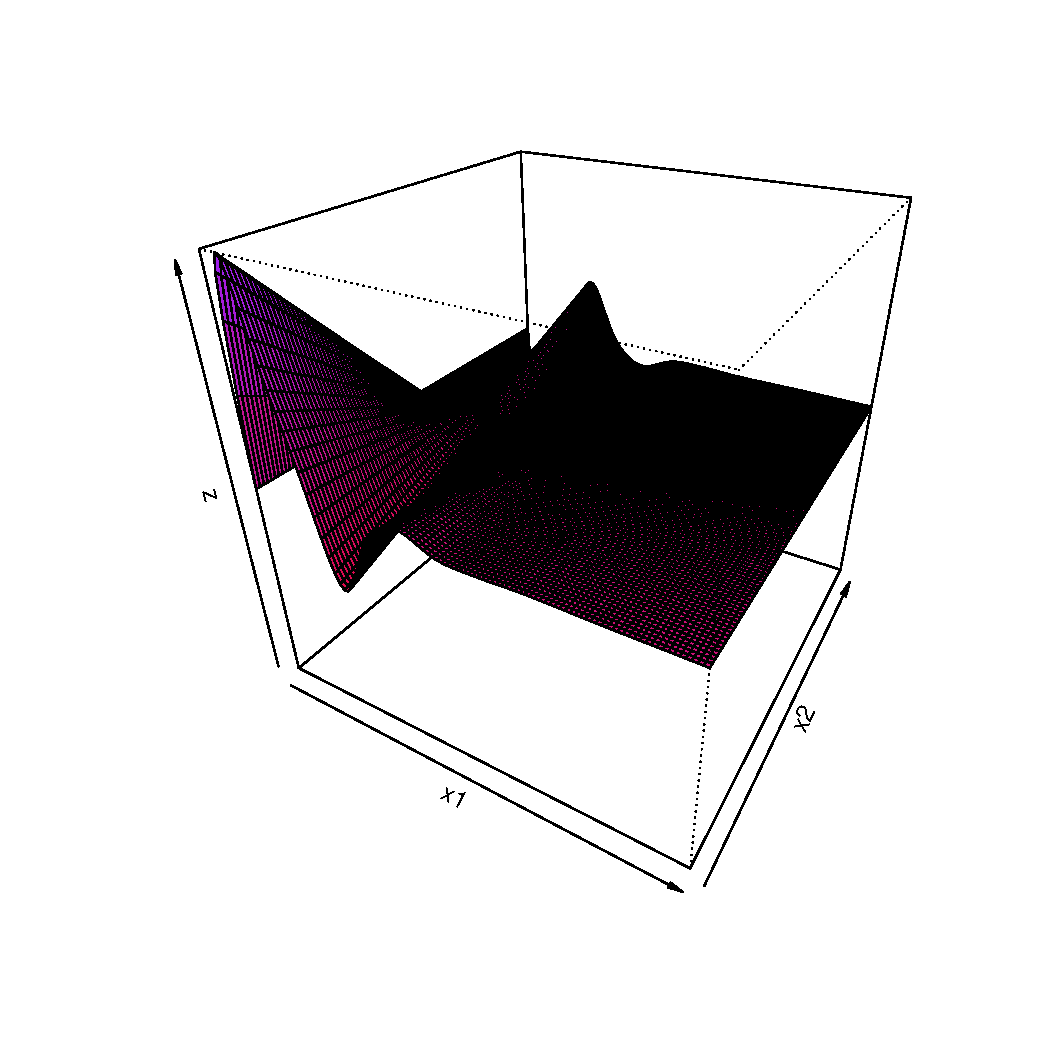
\includegraphics[width=90mm]{fig/salustowitz_col.pdf}
				\caption{Salustowitz function}
				\label{salustowitz}
			\end{figure}
		\subsection{Unwrapped Ball 3D}
			\begin{equation}
				f(x_1, x_2) = \frac{10}{5 + (x_1 - 3)^2 + (x_2 - 3)^2}
			\end{equation}\\
			We can see the plot of the Unwrapped Ball function on the figure \ref{ball}, which is plotted in the 
			ranges as follow:
			\begin{equation}
				\begin{aligned}
				x_1 \in \langle 0, 10 \rangle\\
				x_2 \in \langle 0, 10 \rangle
				\end{aligned}
			\end{equation}
			\begin{figure}
				\centering
				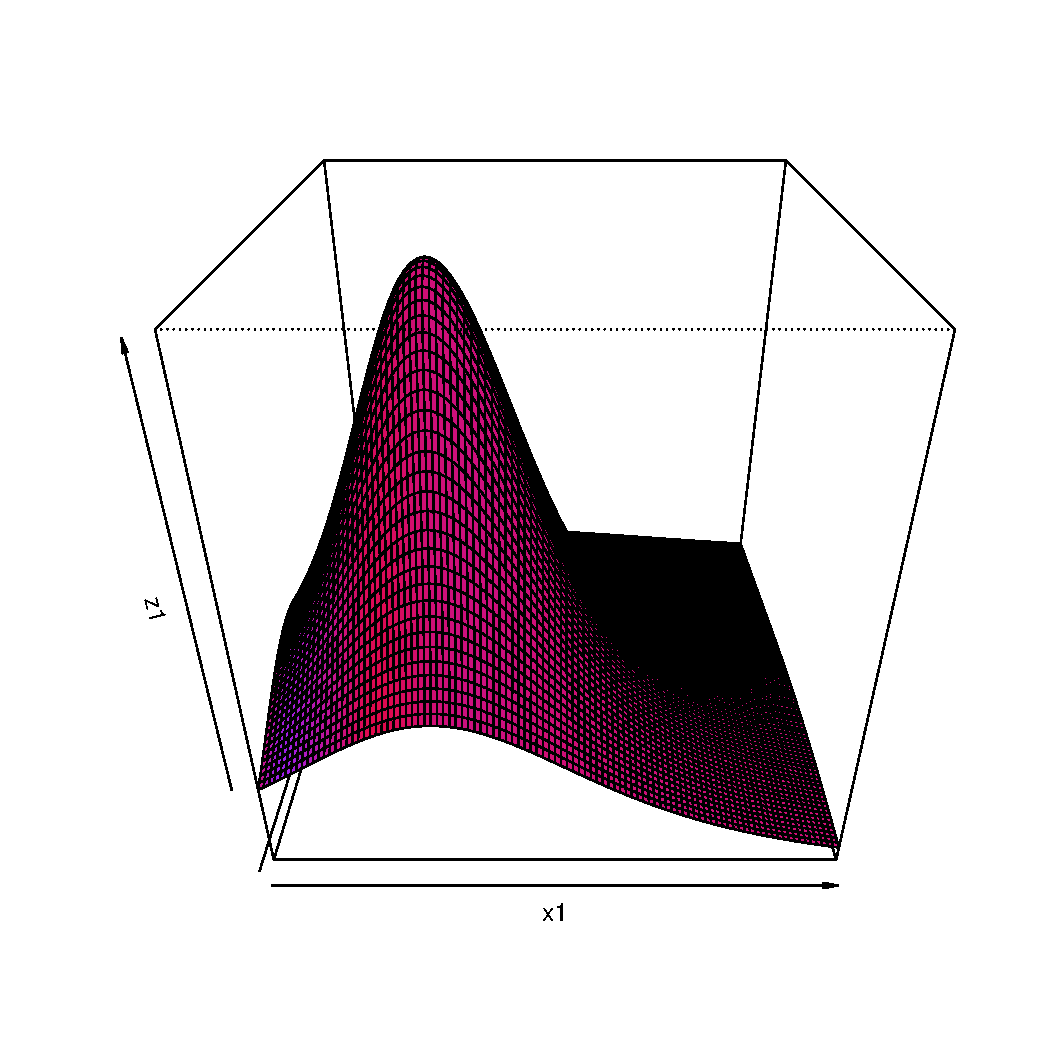
\includegraphics[width=90mm]{fig/unwrapped_ball_col.pdf}
				\caption{Unwrapped Ball function}
				\label{ball}
			\end{figure}

\chapter{Neural network architecture}
	I am going to dedicate this chapter to the architecture of the used neural network. In the 
	beginning I am going to talk about the number of neurons and their organization in the network.
	Then I will speak about the training patterns, how to create and preprocess them, how to make 
	sure that the values will be small enough to be usable for neural network. Then I will speak 
	about the way how I create the data for this specific type of neural network and in the end 
	of the chapter the discussion about activation function, BIAS and other fixed parametres as 
	learning rate will take place.

	\section{Perceptron}

		\begin{figure}
			\centering
			
\includegraphics[width=130mm]{fig/perceptron.jpg}
			\caption{Neural network architecture}
			\label{perceptron}
		\end{figure}\\

		Each neuron in designed neural network works as a simple perceptron. Let's describe a work of
		a perceptron. Schematic picture of perceptron is on the picture \ref{perceptron}. In a general case,
		neuron receives vector x as an input. Each component of the vector (so called characteristic
		value of the vector) is multiplied by factor w (weight) and is added together with remaining
		characteristic values of the vector and with coefficient called bias as well. Bias can also be often seen 
		realized as an unit input multiplied by coefficient $b$.\\

		Output of each perceptron is set by following equation:

		\begin{equation}
			out = act.function \left( \sum w_i x_i + bias \right)
		\end{equation}\\

		In this equation activation function is one of the used functions, as defined below, in the chapter
		\ref{act_funcs}. Sum goes through all the inputs of the neuron, each weighted.\\

		A neural network consists of a set of neurons that are connected to each other and the identity 
		of the connection is determined by the weight w. In multilayer neural networks, there are different 
		layers, where each consists of a set of neurons. It must be mentioned 
		that in a neural network is not necessary the number of neurons of each level to be the same. 
		Also it is not necessary all neurons to implement the same transfer function.\\

		The training of a neural network is to regulate 
		the network connections in order to implement a particular function, and the network to give or 
		to reach/approach a desired output. The arrangement of the connections is done by adjusting the 
		weights. Goal of the network’s training is also the setting of biases. \cite{Eberhartc2007}

	\section{Architecture}
		As it is already proven in the publication \cite{varacha2006}, if you are working on symbolic
		regression throught neural networks, you can use several different neural networks. As a best suitable
		network for 3D functions was found a network with two inputs, one output (as the function requires)
		and two layers (which mean one hidden layer). We can see this neural network on the picture \ref{n_net}.
		\begin{figure}
			\centering
			
\includegraphics[width=130mm]{fig/network.jpg}
			\caption{Neural network architecture}
			\label{n_net}
		\end{figure}\\
		On this picture (\ref{n_net}) we can see a neural network, where individual layers are 
		distincted by shades of grey. The darker shade is for the first layer, the input layer, which 
		doesn't count any functions. It just takes the input and passes it to the next layer. With the
		lighter shade of grey I drawed the hidden and the output layer. \\

		As we can see on the picture, there are 4 active neurons, each of them has a BIAS and inputs.
		Neurons in the hidden layer have two inputs, neurons in the output layer have three inputs. 
		If we count one weight for each input and BIAS for each neuron, we can say, that the state
		of learning of our neural network can be expressed as 13 values. If we give numbers from 
		up to down and from left to right and use the numbers of both connected nodes as an index for
		each weight, we can describe whole neural network by vector of 13 dimensions as follow:

		\begin{equation}
			net = [w_{13}, w_{23}, w_{14}, w_{24}, w_{15}, w_{25}, w_{36}, w_{46}, w_{56}, B_3, B_4, B_5, B_6]
		\end{equation}

	\section{Inputs}
		About inputs of the neural network is known, that it should be small numbers. In the neural networks
		classes we were working with numbers belonging to the interval $\langle 0, 1 \rangle$. In order to
		be in consent with our classes I will continue in keeping the inputs in small numbers. \\

		As I defined before, in the chapter \ref{benchmarks}, I am testing the neural network on two 
		functions, both of them defined on the same interval. Some of my inputs can look like this:

		\begin{equation}
		\label{input_vector}
			[3, 5.7]
		\end{equation}\\

		It it not in the shape how it is suitable for neural network, so I will do a mathematical 
		transformation for my input vector in order to keep the values small. As my inputs are always
		in the interval $\langle 0, 10 \rangle$, to get it into the interval $\langle 0, 1 \rangle$,
		I will do the simple operation: divide all the inputs by 10. The input vector defined in the 
		equation \ref{input_vector} will now look like this:
		\begin{equation}
			[0.3, 0.57]
		\end{equation}		

	\section{Outputs}
		In the previos chapter we have been speaking about the transformation of data on the input 
		of the neural network. We decided to divide all the data we put into the network by 10.
		Of course we are still looking for the same function, but on 10 times smaller domain, so
		we have to recount desired outputs for all input patterns. \\

		This means, that we are creating completely new set of patterns, which fits better the 
		neural network learning process. After we finish learning, we can take input from any
		part of whole domain and make it a new pattern in order to test if the neural network 
		found solution which is suitable for whole domain.

	\section{Generating data}
		The best way of generating training and testing patterns for our networks is doing it 
		automatically in some supporting software. The way of creating it depends on the way how
		we want to run our neural network application. In case we have got the neural network
		learning function as a binary file and run it from operating system on our computer, 
		the best way to keep our data is in a data file. We can load the data from a data file in
		every run. Other way is designing the application of neural networks directly for the problem 
		which we are trying to solve. In that case we can write the training patterns directly into 
		the code of our application.\\

		For our application we are using MATLAB script file, which is designed for our specific
		task, so we can write the data statically into the data vector in the beginning of the code. \\

		For both cases, it is useful to generate the data automatically, code used for generation
		of data for our second testbench could look like it is shown in the algorithm \ref{ahh}.\\

		\begin{algorithm}
			\SetAlgoLined
			\SetKwFunction{generate}{data generation}
			\generate{}\\
				\Begin{\
				y = 0\;
				\For{x = 0; x != 10 ; x += 0.1}{
					y += 0.1\;
					write(x)\;
					write(y)\;
					write(10 / (5 + (x - 3)^3 + (y - 3)^2))\;\\
					write(newline)\;\\
				}
			}\
			\caption{Data generation algorithm}
			\label{ahh}
		\end{algorithm}

	\section{Activation functions}
	\label{act_funcs}
		In neural networks we use activation functions to correct the output of each neuron to keep
		it in the interval, where we want to have it. The most known functions and functions which we 
		are using in our lessons are hard limit function (so called step function), pure linear 
		function and sigmoid function. Their graphs are displayed on the figure \ref{activation_funcs}.\\

		\begin{figure}
			\centering
			\subfloat[][Hard limit function]{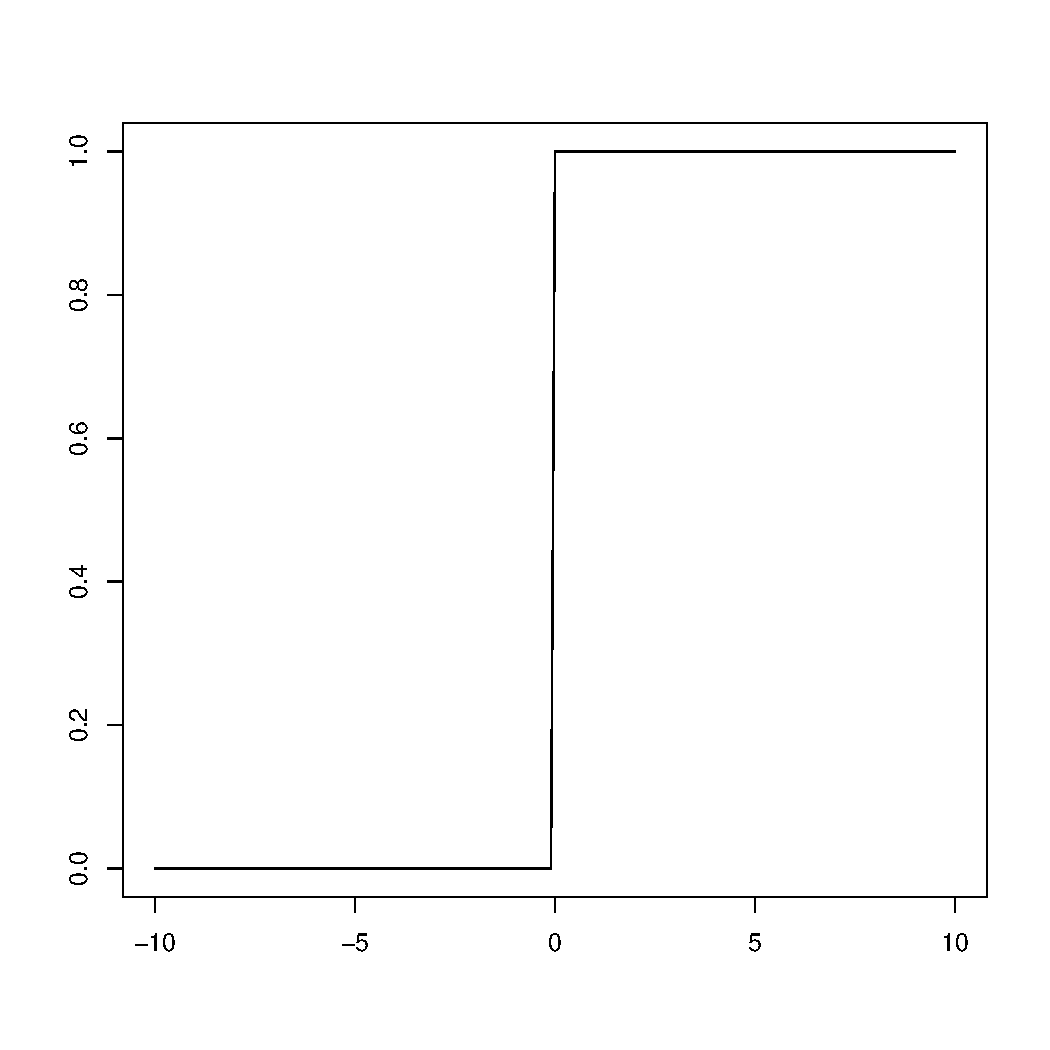
\includegraphics[width=60mm]{fig/hardlim.pdf}}
			\subfloat[][Linear function]{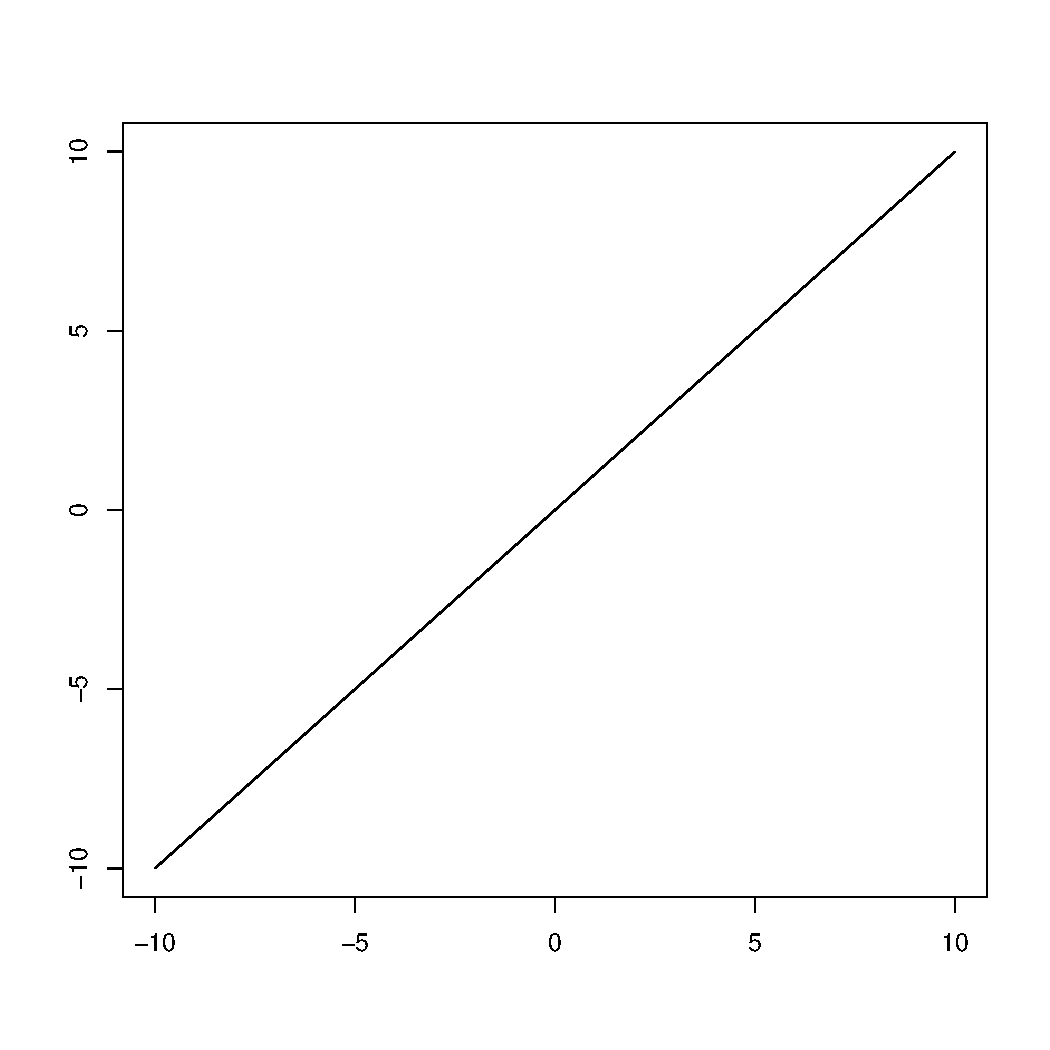
\includegraphics[width=60mm]{fig/linear.pdf}}\\
			\subfloat[][Sigmoid function]{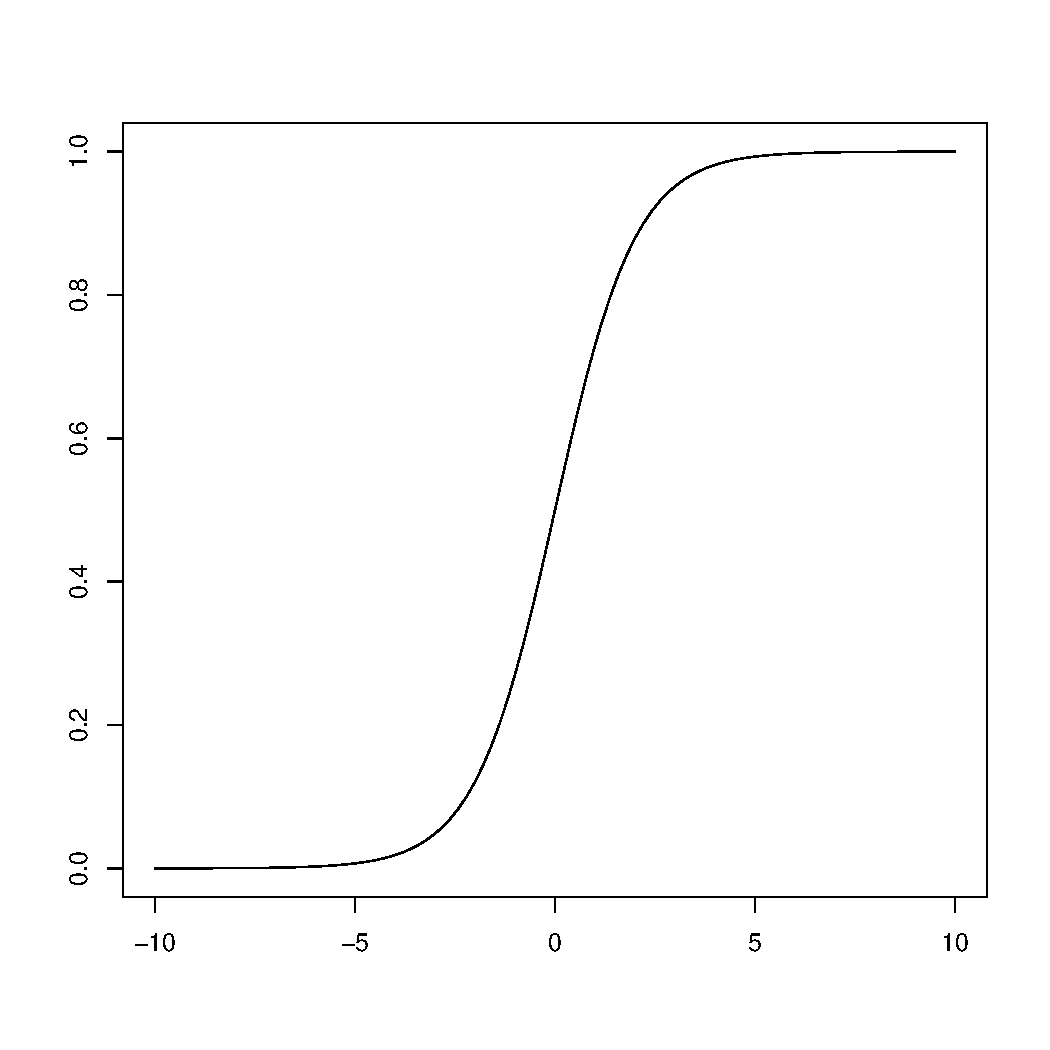
\includegraphics[width=60mm]{fig/sigmoid.pdf}}
			\caption{Used activation functions.}
			\label{activation_funcs}
		\end{figure}

		In the neural networks application which is described in this project, it was decided to use two
		types of activation functions. For all neurons in the hidden layer we are using sigmoid
		activation function in order to keep the values small. For the neuron in the output layer
		we are using linear activation function. The harm limit activation function doesn't have its
		place in this application. It is caused by the type of the problem. Hard limit function is 
		usually use in the problems of a classificatory character in order to separate patterns belonging
		to one group (e.g. 0) from patterns belonging to the other group (e.g. 1). \cite{Papavasileiou2014}

	\section{Other parameters}
		Parameters, which I am going to discuss in this section are mainly the starting values of all
		trained magnitudes. Due to the fact, that the application uses also evolutionary algorithms 
		in order to train the network, the initial weights and biases are set randomly, as it is usual
		in evolutionary algorithms for initial population.

	\section{Lerning algorithms}
		In the application there were used three types of learning process:
		\begin{enumerate}
			\item Backpropagation algorithm
			\item Nonlinear interlacing
			\item SOMA algorithm
		\end{enumerate}\\

		Knowledge from our course covers only one of them in detail, so I decided to devote this
		project mainly to backpropagation algorithm and a way of learning through it. Weights updating 
		in backpropagation algorithm can work in two different ways:
		\begin{description}
			\item [Sequential update] - sequential (so called online) update means, that every time we let one pattern go through
			a network, we count error, which gives us necessary values for counting the $\delta$ (deltas)
			of the output layer, and then we continue backwards until we get to the first layer. Then,
			after updating all weights, we load the next pattern to repeat whole procedure.
			\item [Batch update] -  this type of update means, that as a first task, we count errors 
			and deltas for all patterns. After that, we count an average delta and count the weight 
			changes only once, after counting all patterns with initial weights. 
		\end{description}\\

		In application which I have chosen for this project, the online update version of this algorithm 
		is used. For completeness, let's now define equations used in the backpropagation algorithm \cite{Papadourakis2014}.

		\begin{equation}
			\label{output_layer}
			\delta_k = o_k (1 - o_k)(t_k - o_k)
		\end{equation}
		\begin{equation}
			\label{hidden_layer}
			\delta_h = o_h (1 - o_h) \displaystyle\sum_{k \in outputs} w_{h, k}\delta_k
		\end{equation}
		\begin{equation}
			\label{weight_updates}
			\begin{aligned}
			w_{i, j} = w_{i, j} + \delta w_{i, j}\\
			\Delta w_{i, j} = \eta \delta_j x_{i, j}
			\end{aligned}
		\end{equation}\\

		The equation \ref{output_layer} is counted for each output unit $k$, the equation \ref{hidden_layer}
		is valid for all hidden units with number $h$. The set of equations \ref{weight_updates} is used
		for updating weights after all.

\chapter{Results}
	Result of this application is to prove that neural networks are able to solve this kind of problem 
	succcesfully. In the application which I am starting from, the author was using two basic 3D functions, 
	which are shown on plots \ref{his_testbenches}. Equations according to this functions are
	following.

	\begin{equation}
		f(x_1, x_2) = 0.5 x_1 + 2 x_2
	\end{equation}
	\begin{equation}
		f(x_1, x_2) = 0.5 x_1^6 + 2 x_2^3
	\end{equation}\\

	The results of used functions are shown in the table \ref{results_table_orig}. Tests were done on the same
	set as was training. Success was measured in standard deviation from the desired value.\\

	As an experiment, I am now trying to estimate error, which can be reached on my tesbenches. 
	My estimations come out from comparsion of the linear and polynomic functions next to Salustowitz
	and Unwrapped Ball functions in cartesian genetic programming with coevolution. As I said before, the
	success rate is much worse in these much more dificult functions. As an experimental result, I framed
	the table \ref{results_table_my} to predict awaited results. To prove if the errors which this 
	neural network really reaches are corresponding to my predictions, we will need to do more 
	research and testing. 

	\begin{table}
		\centering
		\begin{tabular}{l | r}
			\hline
			$f_{linear}$ & 10^{-3} \\ \hline
			$f_{polynom}$ & 10^{-6}\\ \hline
		\end{tabular}
		\label{results_table_orig}
		\caption{Application results}
	\end{table}\\

	\begin{table}
		\centering
		\begin{tabular}{l | r}
			\hline
			$f_{Salustowitz}$ & 10^{-5} - 10^{-2} \\ \hline
			$f_{Unwrapped Ball}$ & 10^{-2} - 10^{-1}\\ \hline
		\end{tabular}
		\label{results_table_my}
		\caption{Predicted results for my testbenches}
	\end{table}\\

	As it was proven in
	\cite{vsikulova2012coevolution}, the success rate (number of succesful solutions from 100)in basic 
	linear or polynomial functions is 1.25 times worse in the Salustowitz function (our testbench no. 1)
	and 4 times worse in the Unwrapped Ball function.

	\begin{figure}
		\centering
		\subfloat[][Linear 3d function]{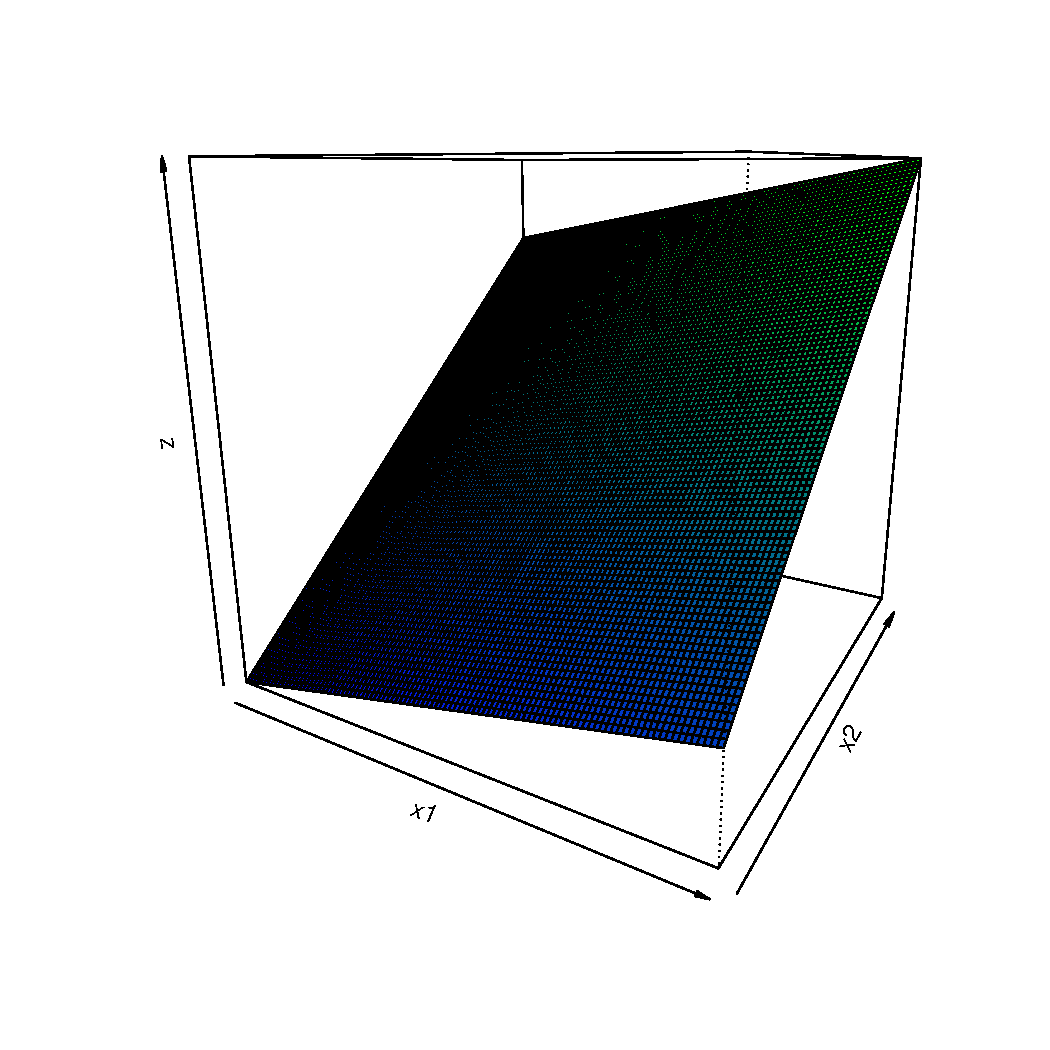
\includegraphics[width=60mm]{fig/linear3d.pdf}}
		\subfloat[][Polynomial 3d function]{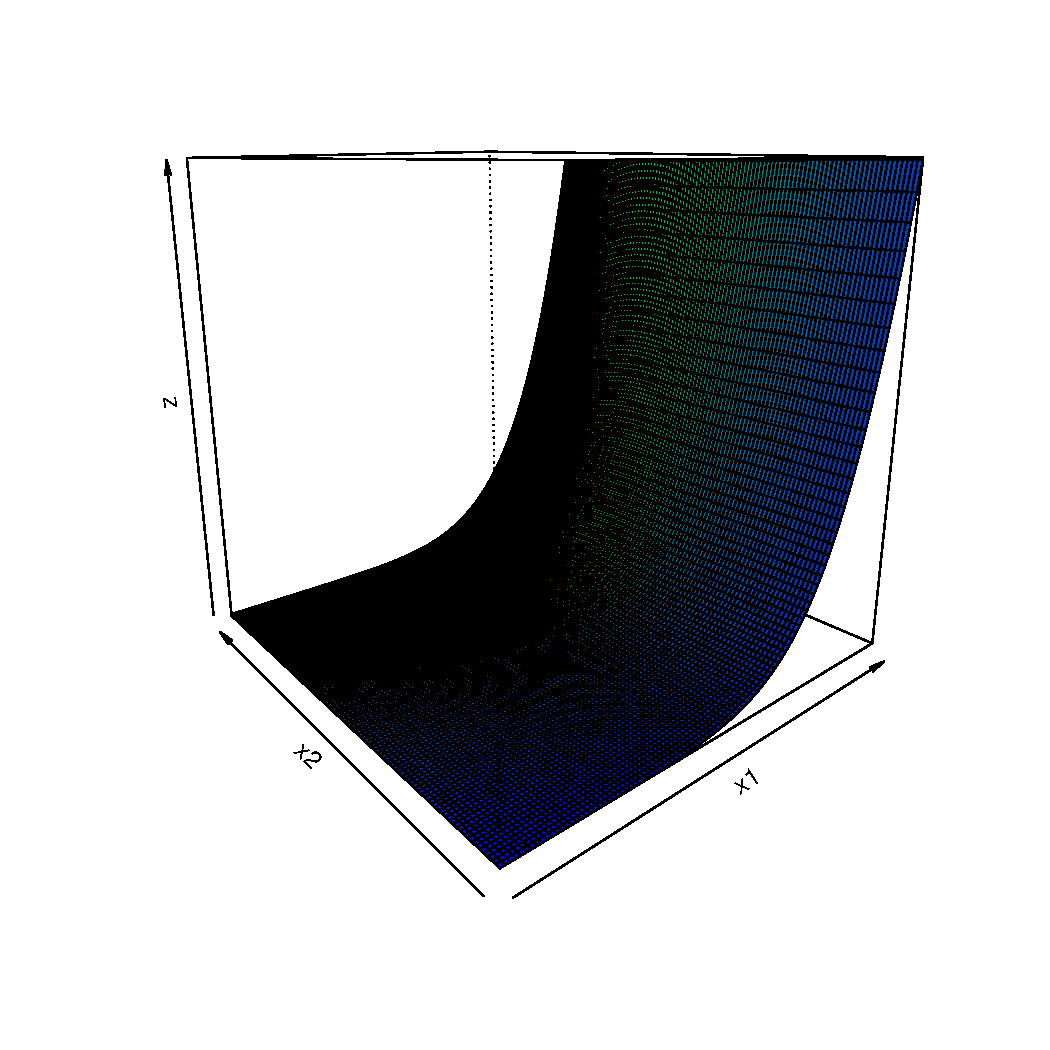
\includegraphics[width=60mm]{fig/polynom.pdf}}
		\caption{Testbenches used in original application}
		\label{his_testbenches}
	\end{figure}

\chapter{Conclusions}
	In this project I described the symbolic regression problem in general, I found an application on the
	internet which deals with symbolic regression realized by neural networks. It is an application of 
	the character of proving that it is possible to solve symbolic regression with neural networks. \\

	I also introduced the application which deals with symbolic regression by cartesian genetic programming
	(CGP) using coevolution. As this two ways of programming are very close, due to both of them are parts of
	main streams in artificial intelligence, I decided to presume, that the ratio of success will be analogic
	in both of them. So I started from ratio between problems solved by application which I was talking about
	and problems which I set to solve by neural networks and were already solved by CGP. I used the ratio which
	was reached by CGP to predict how good will be the application of neural networks for the same problem. \\

	In this project, I was trying to describe the problem completely from basic theories well-founded by equations,
	pictures and 3D plots. I continued with my estimations of the following results of research. During working 
	on this project, I made a complete overview of using basic neural networks for solving problems and how it is
	executed.

\bibliographystyle{plain}
\begin{flushleft}
\bibliography{literatura} % viz. literatura.bib
\end{flushleft}
\appendix

\end{document}
%=========================================================================